\documentclass[draft]{aiaa-tc}% insert '[draft]' option to show overfull boxes

 \usepackage{varioref}%  smart page, figure, table, and equation referencing
 \usepackage{wrapfig}%   wrap figures/tables in text (i.e., Di Vinci style)
 \usepackage{threeparttable}% tables with footnotes
 \usepackage{dcolumn}%   decimal-aligned tabular math columns
  \newcolumntype{d}{D{.}{.}{-1}}
 \usepackage{nomencl}%   nomenclature generation via makeindex
%  \makeglossary
  \makenomenclature
 \usepackage{subfigure}% subcaptions for subfigures
 \usepackage{subfigmat}% matrices of similar subfigures, aka small mulitples
 \usepackage{fancyvrb}%  extended verbatim environments
  \fvset{fontsize=\footnotesize,xleftmargin=2em}
 \usepackage{lettrine}%  dropped capital letter at beginning of paragraph
 \usepackage[dvips]{dropping}% alternative dropped capital package
 \usepackage[colorlinks]{hyperref}%  hyperlinks [must be loaded after dropping]

 \title{Genetic Optimization of Fuzzy Logic Control for Coupled Dynamic Systems}

 \author{
  Andrew Janson, %\thanks{Computer Science, College of Engineering and Applied Science, Address, and AIAA Member Grade.}
  Nicklas Stockton, %\thanksibid{1}\\
  and Kelly Cohen\\
  {\normalsize\itshape
   College of Enginering and Applied Science, University of Cincinnati, Cincinnati, Ohio}}

 % Data used by 'handcarry' option
 \AIAApapernumber{??}
 \AIAAconference{SciTech, 5 January 2015, Kissimmee, FL}
 \AIAAcopyright{\AIAAcopyrightD{YEAR}}

 % Define commands to assure consistent treatment throughout document
 \newcommand{\eqnref}[1]{(\ref{#1})}
 \newcommand{\class}[1]{\texttt{#1}}
 \newcommand{\package}[1]{\texttt{#1}}
 \newcommand{\file}[1]{\texttt{#1}}
 \newcommand{\BibTeX}{\textsc{Bib}\TeX}

\begin{document}

\maketitle

\begin{abstract}
This research project, in the field of control systems, was funded by the National Science Foundation through the Research Experience for Undergraduate (REU) students. The objective of this project was to combine the robustness of fuzzy logic control with the adaptability of genetic algorithms to produce a self-optimizing oscillation damping control mechanism. Once an initial fuzzy inference system (FIS) is developed by an expert for a given dynamic system, the genetic algorithm will be able to optimize the FIS for a range of similar systems with varying parameters. In order to evaluate the control mechanisms developed during this project, a simulation of a two cart spring-mass system was developed in MATLAB. The performance of the controllers was determined by how quickly it could approach a wall and how close it was able to settle the car system to the wall without crashing. The membership functions of the FIS were reduced to an array of real-valued parameters in order to be used in a genetic algorithm. Once the genetic representation of the FIS was defined, the selection, reproduction, and mutation methods were developed to complete the genetic algorithm. The best solution developed by the genetic algorithm was evaluated against the hand-tuned solution developed in the first phase of the project. In order to simulate varying parameters between similar dynamic systems, the mass of the car system in the simulation was varied from 3kg to 20kg. For each weight change the genetic algorithm was allowed to re-optimize the parameters of the FIS. The performance of the genetic algorithm, with respect to the theoretical best, varied up to 17\%, while the unmodified FIS varied up to 300\%. These results show that genetic algorithms are necessary to allow fuzzy control mechanisms to adapt to different systems with little external input from a general user.
\end{abstract}

%\printglossary% creates nomenclature section produced by MakeIndex
\printnomenclature
\section{Introduction}\label{sec:intro}

\lettrine[nindent=0pt]{F}{uzzy} logic systems are used as control systems which are capable of handling the vagueness of the real world. Fuzzy logic can model and control nuances overlooked by the binary logic of conventional computers.\cite{kosko:91bk} In fuzzy logic, the truth of any statement becomes a matter of degree. Take for example, determining the timespan of the weekend.\cite{matlab:12tb} Binary logic allows only a yes/no answer to the question: ``Is this day part of the weekend?'' However, human reasoning does not consider the ``weekendness'' of a day to immediately rise to a value of one from zero at exactly 12am Saturday. We usually view most of Friday as a part of the weekend, determined by when we decide to quit working. Fuzzy logic allows us to specify that most of Friday is considered the weekend as well by assigning it a value of less than one but greater than zero. This distinction gives the fuzzy logic system much more robustness compared to binary logic as it can map a larger range of inputs.

Many structural dynamics problems may be represented by a coupled set of second-order dynamic systems. Coupled rigid-body and flexible body dynamics are sensitive to movement vibrations, which add instability to the structures. The best solution is to use active control to augment structural dynamics.
The objective for this research project is to develop an effective non-linear active structural control methodology to provide stability in large flexible structures. Such structures include robotic manufacturing arms that must perform tasks in a quick and accurate manner. This project also takes into consideration managing stability with minimum cost. Stability in these structures is obtained by damping oscillations that occur during rapid movement of the structure.

Optimization of the non-linear fuzzy logic controller is best accomplished using genetic algorithms. Fuzzy logic controllers are defined by a large set of parameters which greatly increase the search space to find optimum values for the controller. Genetic algorithms mimic natural evolution through Darwinian selection [3]. Individuals who are best suited to the environment survive and produce the next generation. Over a large number of generations individuals become stronger as the weaker individuals are filtered out. Starting with a large number of diverse solutions allows for larger portions of the search space to be investigated and to then converge on areas that provide the best solutions. The automation of the optimization process generalizes the fuzzy logic controller so that it may be easily applied to different systems with varying requirements and parameters.
 

\begin{wrapfigure}{R}{0.3\linewidth}
 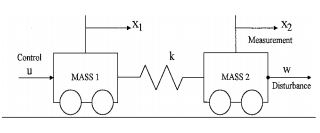
\includegraphics{ACC2}
 \caption{Magnetization as a function of applied field.}
 \label{f:magnetic_field}
\end{wrapfigure}

In an effort to more tightly integrate text and image, the
\package{wrapfig} package is employed.
This package works by modifying paragraph shape to accommodate a figure
(or a table or other items).
Typically one inserts its \verb|wrapfigure| or \verb|wraptable|
environment just before the paragraph in which it is to be placed.
Also specified is the width of the item to be inserted and the
placement, for example, left or right side.
(This package does not provide for center placement.)
The rest of this paragraph is filler so that the \verb|wrapfigure|
example will be placed in this paragraph.
Documentation of the \package{wrapfigure} package is available at the
end of the style file itself (check the package loading lines shown
during \LaTeX\ processing to find its location).

Code listings and other such artifacts can be typeset in a large variety
of styles by using the \package{fancyvrb} package.
\begin{Verbatim}[numbers=left]
 def testCircularAdvection
  position.each_index do |i|
   @position = position[i]
   assert_equal speed[i], waveSpeed
  end
 end
\end{Verbatim}

Tables with footnotes, such as table~\vref{t:threepart},
can be coded using the \package{threeparttable} package.
Note: This table was purposely placed on another page through the use of
the \verb|[p]| placement specifier to demonstrate the automated page
reference mechanism provided by the \package{varioref} package.
Of course, one would normally have the table integrated into the text
that describes it.
\begin{table}[p]
 \begin{center}
  \begin{threeparttable}
   \caption{This is an example of a \package{threeparttable} which uses the
     \package{dcolumn} package to allow for columns to be aligned on decimal
     points.}
   \label{t:threepart}
   \begin{tabular}{lcdd}
    First head\tnote{*}  &
    Second head &
    \multicolumn{1}{c}{Third head} &
    \multicolumn{1}{c}{$V_M(r)$} \\\hline
    center & doctor &  0.2  & 10.55 \\  
    tab    & dentist &  0.15 & 33.12 \\ 
    worse  & man\tnote{\ensuremath{\dagger}} & 10.58 & 45.10 \\ 
    better & home & 43.9  & 12.34 \\
   \end{tabular}
   \begin{tablenotes}
    \item[*] This is a table footnote, which to span multiple lines, has
      been greatly extended in length contrary to reason.
    \item[\ensuremath{\dagger}] A much shorter table footnote.
   \end{tablenotes}
  \end{threeparttable}
 \end{center}
\end{table}

Equation~\eqnref{e:displace} is serving as a demonstration of the
\package{nomenclature} package.
\begin{equation}
  \label{e:displace}
  \mathbf{J}_i\cdot\Delta\underline{x}_{i+1}=-\underline{f}_i
\end{equation}%
\nomenclature{$J$}{Jacobian Matrix}%
\nomenclature[b$i$]{$i$}{Variable number}%
\nomenclature[g$\Delta$]{$\Delta x$}{Variable displacement vector}%
\nomenclature{$f$}{Residual value vector}%
\nomenclature{$x$}{Variable value vector}%
The same can be said for Eq.~\eqnref{e:newton} that uses $\alpha$ to add
another Greek letter to the mix.
\begin{equation}
  \label{e:newton}
  F=m\alpha
\end{equation}%
\nomenclature{$F$}{Force, N}%
\nomenclature{$m$}{Mass, kg}%
\nomenclature[g$\alpha$]{$\alpha$}{Acceleration, m/s\textsuperscript{2}}%
The \package{nomencl} package is fed entries with the
\verb|\nomenclature| command.
These entries are then collected and sorted using \verb|makeindex|.
The optional sorting argument to the \verb|\nomenclature| command uses
a key of `b' for subscripts, `g' for Greek symbols, `c' for conventions,
and `t' for superscripts.

When many figures share a similar style and beg to be compared to one
another, the \package{subfigmat} and \package{subfigure} packages can be
used to create a matrix of subfigures as shown by
figure~\vref{f:small_multiple}.
\begin{figure}
 \begin{subfigmatrix}{4}% number of columns
  \subfigure[2 AM.]{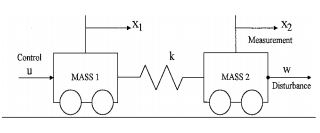
\includegraphics{ACC2}}
  \subfigure[3 AM.]{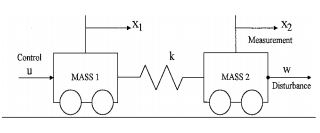
\includegraphics{ACC2}}
  \subfigure[4 AM.]{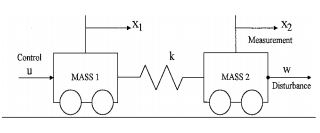
\includegraphics{ACC2}}
  \subfigure[5 AM.]{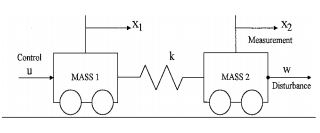
\includegraphics{ACC2}}
  \subfigure[6 AM.]{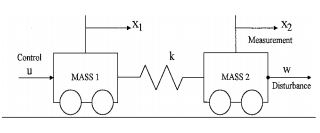
\includegraphics{ACC2}}
  \subfigure[7 AM.]{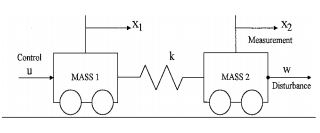
\includegraphics{ACC2}}
  \subfigure[8 AM.]{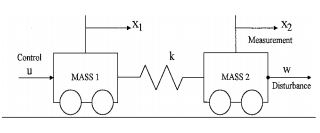
\includegraphics{ACC2}}
  \subfigure[9 AM.]{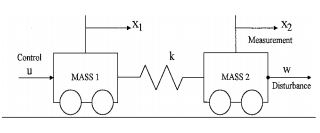
\includegraphics{ACC2}}
 \end{subfigmatrix}
 \caption{A time series shown of magnetic field that does not change
          because we are using the same figure each time.}
 \label{f:small_multiple}
\end{figure}
These are called ``small multiples'' by Tufte.

\section{Conclusion}

This had been a brief example of some of the more advanced options
available for \LaTeX.
Please see the documentation for each package for extended discussion or
usage.

% produces the bibliography section when processed by BibTeX
\bibliography{bibtex_fuzzy}
\bibliographystyle{aiaa}

\end{document}


